\documentclass{article}
\usepackage{subcaption}
\usepackage{float}
\usepackage[utf8]{inputenc}
\usepackage[english]{babel}
\usepackage{amsmath, amssymb}
\usepackage{tikz}
\usepackage{xcolor}
\usepackage{graphicx}
\usepackage{caption}
\usepackage{geometry}
\usepackage[T1]{fontenc}
\usepackage{mathtools}
\geometry{margin=2.5cm}
\title{Modeling of an Algae Pond}
\author{Octave Litrico}
\date{January 2026}

\begin{document}

\maketitle

\section*{Introduction}

In the context of modeling an algae cultivation pond, the evolution of a scalar quantity \( \rho(x,t) \), representing the concentration of algae can be described by a partial differential equation of the advection-diffusion type:

\[
\frac{\partial \rho}{\partial t} + a \frac{\partial \rho}{\partial x} = \mu\frac{\partial^2 \rho}{\partial x^2}
\]

where:
\begin{itemize}
  \item \( a \) is the advection (transport) coefficient related to the movement induced by the water wheel
  \item \( \mu \) is the diffusion coefficient (natural or turbulent dispersion).
\end{itemize}

However, to simplify the numerical analysis and better understand diffusion phenomena alone, we choose in this work to neglect the advection term. This amounts to considering only a pure diffusion equation:

\[
\frac{\partial \rho}{\partial t} = \mu\frac{\partial^2 \rho}{\partial x^2}
\]

\section{The discretized Model}

\subsection{Discretization principle}

Let us discretize the time and space intervals. Let $N, M \in \mathbb{N}$, $h = \Delta_x = \frac{L}{N}, \ \Delta_t = \frac{T}{M}$ and $x_i = i\Delta_x, \ t_n=n\Delta_t \ \forall i \in \{0, \cdots, N\}, n\in \{0, \cdots, M\}$. \\

The pond will be modeled by a rectangle of size $L\times H$ divided into I horizontal layers of same size. The pond is circular, therefore the concentration functions of each layers will have to be periodic with period L. A water wheel located on the x-coordinate $0$ stirs the water and will be modeled by a matrix $P$. It will intervene in the computing of the values of the algae concentration near $0$. So that there is no production nor loss of matter, $P$ must be column-stochastic. Indeed, we have that for all $i, j \in \{1, \cdots, I\}, \ P_{i, j}$ is the amount of matter in line $j$ sent to line $i$. Therefore, we must have that for all $j \in \{1, \cdots, I\}, \ \sum_{k=1}^IP_{k, j} = 1$\\

The concentration function $\rho$ will be an element of \(\mathcal{C}^1([0, T], H^1([0, L])^I)\). At each time \( t_n = n \Delta t \), the concentration in cell \( j\) is denoted \( \rho_j^n = \rho(t_n, x_j)\). \\

\subsection{Cellular automat}

To first understand the underlying motion of the pond, let us introduce a cellular model. With the discretization showed above, we consider a cell in which the algae concentration evolves as a particle. A cell located far from the paddle wheel exchanges mass with its two neighbors. The scheme can be represented as follows:

\begin{center}
\begin{tikzpicture}[scale=1.2, every node/.style={scale=1}]
  \node at (-2,0) {\( v_{i-1}^n \)};
  \node at (0,0) (center) {\( v_i^n \)};
  \node at (2,0) {\( v_{i+1}^n \)};
  
  \draw[->, thick] (-1.6,0.2) -- (-0.4,0.2) node[midway, above] {\( \nu \)};
  \draw[->, thick] (1.6,0.2) -- (0.4,0.2) node[midway, above] {\( \nu \)};
  
  \draw[->, thick] (0.4,-0.3) to[out=300,in=240,looseness=4] (-0.4,-0.4)
    node at (0, -1.5) {\( 1 - 2\nu \)};
\end{tikzpicture}
\end{center}

Here, the value at time \( n+1 \) is a weighted linear combination of the cell and its neighbors. $\nu$ here represents the mass proportion that each cell exchanges. 

\subsection{Special case: near the paddle wheel}

Near the paddle wheel, the stir influences the concentrations. The following scheme represents the evolution, with the wheel located in column 0 :

\begin{center}
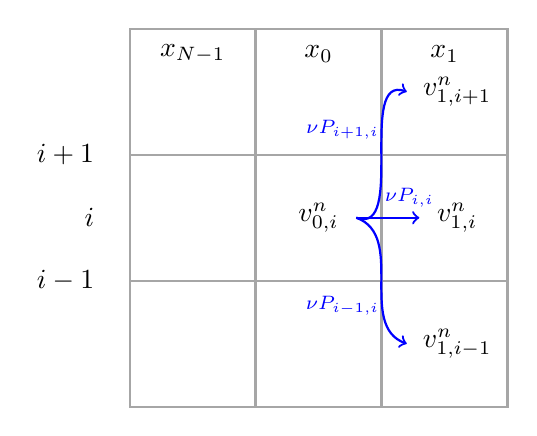
\begin{tikzpicture}[scale=1.6, thick]

    % Grille 3x3
    \foreach \x in {-1,0,1}{
        \foreach \y in {-1,0,1}{
            \draw[gray!70] (\x-0.5,\y-0.5) rectangle (\x+0.5,\y+0.5);
        }
    }

    % Légendes colonnes (placées AU-DESSUS du quadrillage)
    \node at (-1,1.3) {\(x_{N-1}\)};
    \node at (0,1.3) {\(x_0\)};
    \node at (1,1.3) {\(x_1\)};

    % Légendes lignes (sur la gauche)
    \node[left] at (-1.7,0.5) {\(i+1\)};
    \node[left] at (-1.7,0) {\(i\)};
    \node[left] at (-1.7,-0.5) {\(i-1\)};

    % Case centrale
    \node at (0,0) {\(v_{0,i}^n\)};
    \node at (1.1, 0) {\(v_{1, i}^n\)};
    \node at (1.1, 1) {\(v_{1, i+1}^n\)};
    \node at (1.1, -1) {\(v_{1, i-1}^n\)};
    % Flèches incurvées du centre vers la colonne 1
    \draw[->, thick, blue]
        (0.3,0) to[out=-20, in=160] (0.7,-1)
        node at (0.19, -0.7) {\scriptsize \(\nu P_{i-1,i}\)};
    \draw[->, thick, blue]
        (0.3,0) to[out=-20, in=160] (0.7,1)
        node at (0.19, 0.7) {\scriptsize \(\nu P_{i+1,i}\)};
    \draw[->, thick, blue]
        (0.3,0) to (0.8,0)
        node at (0.72, 0.16) {\scriptsize \(\nu P_{i,i}\)};

\end{tikzpicture}
\end{center}


Therefore we end up with this automat : \\
\[\forall n \in \{0, \cdots, M-1\}\]
\[\begin{cases}
    v_j^{n+1} = \nu(v_{j-1}^n + v_{j+1}^n) + (1 - 2\nu)v_j^n \ \ \ \forall j \in \{2, \cdots, N-2\}\\
    v_{N-1}^{n+1} = \nu(v_{N-2}^n + Pv_{0}^n) + (1 - 2\nu)v_{N-1}^n \\
    v_{0}^{n+1} = \nu(v_{N-1}^n + v_{1}^n) + (1 - 2\nu)Pv_{0}^n \\
    v_{1}^{n+1} = \nu(Pv_{0}^n + v_{2}^n) + (1 - 2\nu)v_{1}^n\\
    
\end{cases} \]
 
\section{PDE analysis} 

Let \(\rho(t, x) \in \mathbb{R}^I\) be the vector of algae concentration on the x-coordinate of the pond at time t. We have to take into account the $L-$periodicity :
\[\rho(t, 0) = \rho(t, L) \ \forall t\]

Furthermore, the total algae mass in the pond is constant through time. Therefore, we have : \[\sum_i\int_0^L\rho_i = 0\] up to a translation of the values of the \(\rho_i\) by the average concentration.

Let us denote U the set : \[\{v \in H^2([0, L])^I \ | v(0) = v(L) = Pv(L) \ \text{and} \sum_{i=1}^I(\partial_xv_i(L) - \partial_xv_i(L)) = 0 \}\] \\ and
\[V \text{ an eigen vector of $P$ such that} \ PV = V \ \text{and} \ \|V\|_1 = 1\]
\\ The ponctual values of $\partial_xu$ are well defined. Indeed, thanks to the Morrey injection, we have that $H^2([0, L]) \hookrightarrow
\mathcal{C}^1([0, L])$. 
U is a Hilbert space for the following inner product :
\[<u, v>_{U, U} = \sum_{i=1}^I\frac{1}{V_i}\int_{0}^{L}\partial_x u_i.\partial_x v_i\]

The problem we are looking to solve is :
\[\begin{cases}
    \text{Find}\  \rho \in U \\
    \text{such that} \ \partial_t\rho = \mu \Delta\rho 
\end{cases}\]

Firstly, let us notice that : 
\[
\begin{align}
    &\forall v\in U, \\
    &\langle-\Delta\rho, v\rangle_{U, U} = -\sum_{i=1}^I\frac{1}{V_i}\int_{0}^L\partial_{xx}\rho_iv \\
    &= -\sum_{i=1}^I\frac{1}{V_i}\left[(\partial_x\rho_i(0)v_i(0) - \partial_x\rho_i(L)v_i(L)) - \int_0^L\partial_x\rho_i\partial_xv_i\right]\\
    &= -\sum_{i=1}^I\left(\partial_x\rho_i(0) - \partial_x\rho_i(L) - \int_0^L\partial_x\rho_i\partial_xv_i\right) \quad  \text{because} \ v_i(0) = v_i(L) = V_i  \\
    & = \sum_{i=1}^I\int_0^L\partial_x\rho_i\partial_xv_i
\end{align}
\]

We would like to find a Hilbert basis of $U$ which will ease our difficulties. 
Let us introduce $H = \{h \in L^2([0, L])^I \ |  \sum_i\int_0^Lh_i = 0  \}$, we can easily show that $U$ is dense in H and by using the Rellich theorem, it follows that the embedding of $U$ in $H$ is compact. \\

Let us define for all $u, v \in U$ :
\[ a(u, v) = \mu\sum_{i=1}^I\int_{0}^{L}\partial_x u_i.\partial_x v_i \]

The operator $a$ is symmetric, bilinear, and coercive on $U$ by the Poincaré inequality. Moreover, it is continuous. Therefore, there exists an infinite sequence $(\lambda_n)_n \in \mathbb{N}$ of positive eigenvalues of this operator, and a Hilbert basis $(x \mapsto \rho_n(x))_{n\in \mathbb{N}} \in U^\mathbb{N}$ of H (for the inner product $<.,.>_{H, H}$) of associated eigenvectors. Let's name them $(\rho_n)_{n \in \mathbb{N}}$. The theorem also holds that the sequence $(\frac{\rho_n}{\sqrt{\lambda_n}})$ is a Hilbert basis of U for the inner product $a(., .)$. 

If $\rho$ is solution to (1) then there exists a sequence $(t \mapsto \nu_n(t))_{n \in \mathbb{N}}$ of functions of $H^2([0, T])$ such that:
\[\rho(t, x) = \sum_\mathbb{N}\nu_n(t)\rho_n(x)\]

The values of $\rho_n$ and of $\nu_n$ must be found.

\[-\mu \Delta u = \lambda u \] with $\lambda > 0$
So \[u(x) = A \cos\left(\sqrt{\frac{\lambda}{\mu}}x\right) + B\sin\left(\sqrt{\frac{\lambda}{\mu}}x\right)\] with $A, B \in \mathbb{R}^{I} $

Moreover, we know that $u(0) = Pu(0)$
and that P is irreducible and thus has an eigenspace associated to the eigenvalue 1 of dimension 1. Let us denote V a vector of norm 1 of this space. As each $V_i$ is positive (given the ergodic theorem) we have $\| V \|_1 = \sum_i V_i = 1 $
Then, $A = \alpha V$ with $\alpha \in \mathbb{R}$\\

With $u_i(0) = u_i(L)$ we see that :
\[B\sin\left(\sqrt{\frac{\lambda}{\mu}}L\right) = A\left[1-\cos\left(\sqrt{\frac{\lambda}{\mu}}L\right)\right]\]

If $\sqrt{\frac{\lambda}{\mu}}L \notin \pi \mathbb{Z}$ then :  \[B = \alpha V\frac{(1-\cos(\sqrt{\frac{\lambda}{\mu}}L))}{\sin(\sqrt{\frac{\lambda}{\mu}}L)}\]

Because $\sum_i\int_0^L\rho_i = 0 $we have :
\[ \sum_i\left[A_i\sin\left(\sqrt{\frac{\lambda}{\mu}}L\right) + B_i\left(1- \cos\left(\sqrt{\frac{\lambda}{\mu}}L\right)\right)\right] = 0\]

i.e \[\alpha\left(1-\cos\left(\sqrt{\frac{\lambda}{\mu}}L\right)\right)^{2} = -\alpha\sin\left(\sqrt{\frac{\lambda}{\mu}}L\right)^{2}\]

therefore, as $\alpha \neq 0$ because $u \neq 0$, we have : \[(1-\cos(\sqrt{\frac{\lambda}{\mu}}L))^{2} = - (1-\cos(\sqrt{\frac{\lambda}{\mu}}L)^{2})\]

We end up with the following equation : \[\cos\left(\sqrt{\frac{\lambda}{\mu}}L\right) = 1\]
i.e $\sqrt\frac{\lambda}{\mu}L \in 2\pi\mathbb{Z}$, contradiction.\\

Therefore, $\sqrt{\frac{\lambda}{\mu}}L \in \mathbb{N^*}\pi$\\

$\sqrt{\frac{\lambda}{\mu}}L = n\pi$ with $n \in \mathbb{Z^*}$. 

\begin{itemize}
    \item If $n \in 2\mathbb{N^*} $ then the equation $\sum_i\int_0^L\rho_i = 0$ is trivial, and there is no constraint on the $B_i$.

\item If $n \in 2\mathbb{N^*}  + 1$ then we have :
\[\sum_iB_i = 0\]
and :
\[A(1-\cos(\sqrt{\frac{\lambda}{\mu}}L)) = 2A = 0\] so \[\alpha = 0\]

We have eventually found all the eigen vectors of the operator $a$. These are the elements of the following sets :
\begin{itemize}
    \item \( \{x \mapsto V\cos(\frac{2n\pi x}{L})\}_{n \in \mathbb{N^*}} \)
    \item \( \{x \mapsto e_1\sin(\frac{2n\pi x}{L})\}_{n \in \mathbb{N^*}} \)
    \item \( \cdots \)
    \item \( \{ x \mapsto e_I\sin(\frac{2n\pi x}{L})\}_{n \in \mathbb{N^*}} \)
    \item \( 
        \left\{ x \mapsto \sum_{i=1}^I\gamma_{2n + 1}^{i} e_i\sin(\frac{(2n + 1)\pi x}{L}) \ \middle| \ \sum_{i=1}^{I} \gamma_{2n + 1}^{i} = 0 \right\}_{n \in \mathbb{N^*}}
    \)
\end{itemize}

\end{itemize} 

As shown before, these vectors form a Hilbert basis of $U$ equipped with the inner product $a(., .)$ up to normalization.Therefore we can decompose $\rho$ in this basis : there exist $\mathcal{C}^1([0, T], \mathbb{R}) $ functions  $\alpha_{2n}, \beta_{2n}^{i}, \gamma_{2n+1}^{i} \forall n \in \mathbb{N^*}, i \in \{1, \cdots, I\}$ such that 
\[\rho(x, t) = \sum_{n \in \mathbb{N^*}}\left[ \alpha_{2n}(t)V\cos\left(\frac{2n\pi x}{L}\right) + \sum_{i=1}^{I}\beta_{2n}^{i}(t)e_i \sin\left(\frac{2n\pi x}{L}\right) + \sum_{i=1}^{I}\gamma_{2n+1}^{i}(t)e_i \sin\left(\frac{(2n + 1)\pi x}{L}\right)\right]\] with $\sum_{i=1}^{I}\gamma_{2n+1}^{i}(t) = 0\ \forall t$ \\ \\

Therefore for all $n \in \mathbb{N^*}, i \in \{1, \cdots, I\}$, $\alpha_{2n}, \beta_{2n}^{i}, \gamma_{2n+1}^{i}$ satisfy the respective equations \[\begin{cases}
\alpha_{2n}'(t) = \frac{-4n^2\pi^2\mu}{L^2}\alpha_{2n}(t)\\
{\beta_{2n}^{i}}'(t) = \frac{-4n^2\pi^2\mu}{L^2}\beta_{2n}^{i}(t)\\
{\gamma_{2n+1}^{i}}'(t) = \frac{-(2n + 1)^2\pi^2\mu}{L^2}\gamma_{2n+1}^{i}(t) 
\end{cases}
\text{for all}\ t \in [0, T]\]

Therefore, 

\[
\begin{cases}
\alpha_{2n}(t) = \alpha_{2n}(0)\, e^{\frac{-4n^2\pi^2\mu}{L^2} t} \\
\beta_{2n}^{i}(t) = \beta_{2n}^{i}(0)\, e^{\frac{-4n^2\pi^2\mu}{L^2} t} \\
\gamma_{2n+1}^{i}(t) = \gamma_{2n+1}^{i}(0)\, e^{\frac{-(2n + 1)^2\pi^2\mu}{L^2} t}
\end{cases}
\quad \text{for all } t \in [0, T]
\] \\

Furthermore, as for all $n \in \mathbb{N^*}, i \in \{1, \cdots, I\}$ we have :
\[\rho_0(x) = \sum_{n \in \mathbb{N^*}}\left[ \alpha_{2n}(0)V\cos(\frac{2n\pi x}{L}) + \sum_{i=1}^{I}\beta_{2n}^{i}(0)e_i \sin(\frac{2n\pi x}{L}) + \sum_{i=1}^{I}\gamma_{2n+1}^{i}(0)e_i \sin(\frac{(2n + 1)\pi x}{L})\right]\] \\

with for all $n \in \mathbb{N}^*$:
\[
\begin{cases}
    \alpha_{2n}(0) = \frac{2}{L\|V\|_2^2}\int_0^L\rho_0(x)\cdot V\cos(\frac{2n\pi x}{L})dx  \quad \text{for a certain} \ V_j \neq 0 \\
    \beta_{2n}^i(0) = \frac{2}{L}\int_0^L\rho_0(x)\cdot e_i\sin(\frac{2n\pi x}{L})dx \\
    \gamma_{2n + 1}^i(0) = \frac{2}{L}\int_0^L\rho_0(x)\cdot e_i\sin(\frac{(2n+1)\pi x}{L})dx
\end{cases}
\]
The coefficients $\alpha, \beta \ \text{and} \ \gamma$  are imposed by the initial condition. We have therefore found the unique solution to (1).



\section{Convergence of the cellular model}

\subsection{Numerical scheme of the PDE}

We are looking for an approximation of the exact solution $\rho$. We denote $\rho_j^n = \rho(t_n, x_j)$ and $\rho_h^n = (\rho_0^n, \rho_1^n, \ldots, \rho_{N-1}^n)^T$\\

In this section, we impose that $P$ must be irreducible, so that there exists a unique vector V such that :
\[ \|V\|_1 = 1, V_i \geq 0 \ \forall i \ \text{and} \ PV = V\] \\
Using the expression of the discrete Laplacian and time derivative, we end up with this scheme :   \\

\[
\begin{cases}
\displaystyle
\frac{v_{j}^{\,n+1} - v_{j}^{\,n}}{\Delta_t}
- \mu\,\frac{v_{j+1}^{\,n} - 2v_{j}^{\,n} + v_{j-1}^{\,n}}{\Delta_x^2} = 0,
& \forall\, j \in \{1,\dots,N-1\},\ n \in \{0,\dots,M-1\}, \\[8pt]

\displaystyle
\sum_{i=1}^I \left(\frac{v_{1,i}^{\,n} - v_{0,i}^{\,n}}{\Delta_x}
- \frac{v_{0,i}^{\,n} - v_{N-1,i}^{\,n}}{\Delta_x}\right) = 0,
& \forall\, n \in \{0,\dots,M-1\}, \\[8pt]

v_{0}^{\,n} = v_{N}^{\,n}, & \forall\, n \in \{0,\dots,M\}, \\[4pt]

P v_{0}^{\,n} = v_{0}^{\,n}, & \forall\, n \in \{0,\dots,M\}.
\end{cases}
\]



We can show that it is equivalent to :\\
\\
$\forall n \in \{0, \cdots, M-1\}$\\
\[
\begin{cases}
    v_j^{n+1} = \nu(v_{j-1}^n + v_{j+1}^n) + (1 - 2\nu)v_j^n \ \ \ \forall j \in \{1, \cdots, N-2\}\\
    v_{N-1}^{n+1} = \nu(v_{N-2}^n + v_{0}^n) + (1 - 2\nu)v_{N-1}^n \\
    v_0^n = \alpha^n V \ \text{with} \ \alpha^n = \frac{1}{2}(\sum_{i=1}^Iv_{1,i}^n + v_{N-1, i}^n)
\end{cases} \\
\]

 
\subsection{Consistency, Stability and Convergence Analysis}

We now show that the cellular model defined in the previous section is consistent and stable in the discrete $L^2$ norm, and therefore convergent toward the continuous diffusion equation.

\paragraph{Discrete notation.}

For each time index $n$, we collect the discrete unknowns in a vector
\[
v_h^n = (v_0^n, v_1^n, \ldots, v_{N-1}^n)^T \in \mathbb{R}^{I N},
\]
where each component $v_j^n \in \mathbb{R}^I$ represents the concentrations of the $I$ layers at node $x_j$.
The discrete $L^2$ inner product and norm are defined by
\[
(u_h, v_h)_h = \Delta_x \sum_{j=0}^{N-1} (u_j^T v_j), \qquad
\|u_h\|_h = (u_h, u_h)_h^{1/2}.
\]

\paragraph{Matrix form of the scheme.}
The fully discrete explicit scheme can be written compactly as
\begin{equation}\label{eq:matrix_scheme}
v_h^{n+1} = Q v_h^n,
\end{equation}
where $Q$ is a block matrix of size $IN\times IN$ that includes:
\begin{itemize}
  \item the tridiagonal coupling due to horizontal diffusion with coefficients $(\nu, 1-2\nu, \nu)$,
  \item the boundary connections involving the matrix $P$.
\end{itemize}

\paragraph{Consistency.} 
\textcolor{red}{We haven't shown the constistency at this point.}
Let $\rho$ be a sufficiently exact solution of the continuous diffusion equation.  
We insert $\rho$ into the discrete scheme to obtain the local truncation (consistency) error:
\[
\tau_j^n =
\frac{\rho(x_j, t_{n+1}) - \rho(x_j, t_n)}{\Delta_t}
- \mu\,\frac{\rho(x_{j+1}, t_n) - 2\rho(x_j, t_n) + \rho(x_{j-1}, t_n)}{\Delta_x^2},
\qquad j = 2, \dots, N-2.
\]
For the interior nodes, the Taylor expansion of $\rho$ in $t$ and $x$ around $(x_j,t_n)$ gives
\begin{equation}
\tau_j^n = 
\frac{\Delta_t}{2}\,\partial_{tt}\rho(x_j, t_n)
- \frac{\mu\,\Delta_x^2}{12}\,\partial_{x^4}\rho(x_j, t_n)
+ \mathcal{O}(\Delta_t^2 + \Delta_x^4), \tag{*}
\end{equation}

But we haven't shown that this also holds for the boundary nodes. $\tau_0^n, \tau_1^n$ and $\tau_{N-1}^n$ are subject to the same approximation.

Let us assume that $(*)$ holds for every value of j. 
Hence for a certain $C>0$ independent of N and M :
\[
\|\tau_j^n\|_2 \leq C(\Delta_t + \Delta_x^2)
\quad \text{for all } n \in \{0, \cdots, M-1\}, \ j \in \{0,\cdots,N-1\}.
\]
Therefore,
\[
\sup_{0 \le n \le M}\|\tau_h^n\|_h \le C\,(\Delta_t + \Delta_x^2),
\]
and the scheme is \textbf{consistent of order $(1,2)$}.


so the scheme is first order in time and second order in space.  
This proves the consistency of the method.

\paragraph{Stability in the discrete $L^2$ norm.}
It is easy to establish that the matrix $Q$ satisfies
\[
\|Q^n\|_2\le 1
\qquad \text{for all } n \ge 0,
\]
provided that the classical CFL condition
\begin{equation}\label{eq:cfl}
0 < \nu = \frac{\mu \Delta_t}{\Delta_x^2} \le \frac{1}{2}
\end{equation}
is fulfilled.
The scheme is stable.


\paragraph{Convergence.}

Let us define the global error $e_h^n = v_h^n - \rho_h^n$.  
From the scheme and the consistency relation, we obtain
\[
e_h^{n+1} = Q e_h^n + \Delta_t\,\tau_h^n.
\]
Iterating and applying the discrete norm gives
\[
\|e_h^{n+1}\|_h \le \|Q^{n+1}\|\|e_h^0\|_h 
      + \Delta_t \sum_{m=0}^{n}\|Q^{n-m}\|\|\tau_h^m\|_h.
\]
Using $\|Q^k\|\le1$ and $e_h^0=0$,
\[
\|e_h^{n+1}\|_h \le T\,\sup_m \|\tau_h^m\|_h
       \le C\,T(\Delta_t + \Delta_x^2).
\]
Thus, if it is consistent, the scheme is convergent of order $\mathcal{O}(\Delta_t + \Delta_x^2)$ in discrete $L^2$ norm.


\section{Numerical study of the convergence}
Let us examine the convergence of the cellular model for three simple
cases: a three-layer basin, with initial functions corresponding to the
system's own functions. We will limit ourselves to cases where 
the coefficients $\alpha_{2k}, \beta_{2k}^i, \gamma_{2k+1}^i$ are zero if and only if
$k = 1$.
Let us take the simple examples of initial functions corresponding to the system's eigen values.
That is functions of the same form as $\rho$ in section 2, with :

\begin{itemize}
    \item  $\alpha_{2k} = \delta_{k, 1}, \ \beta_{2k}^i = 0, \ \gamma_{2k+1}^1 = \gamma_{2k+1}^2 = \gamma_{2k+1}^3 = 0$.
    \item  $\alpha_{2k} = 0, \ \beta_{2k}^i = \delta_{k, 1}, \ \gamma_{2k+1}^1 = \gamma_{2k+1}^2 = \gamma_{2k+1}^3 = 0$.
    \item  $\alpha_{2k} = 0, \ \beta_{2k}^i = \delta_{k, 1}, \  \gamma_{3}^1 = \gamma_{3}^2 = 1 \text{and} \gamma_{3}^3 = -2\gamma_{2k+1}^1 = \gamma_{2k+1}^2 = \gamma_{2k+1}^3 = 0 \forall k \neq 0$.
\end{itemize}

\section{Mixing Optimization : Optimal Matrix}

I have developed a numerical algorithm to model algal growth in a water basin. 
The model is based on the introduction of a source term into the discretization of the advection--diffusion equation with an upwind discretization of the advection term. 

Let us first introduce the numerical scheme.
Far from the paddle wheel, the PDE discretization leads to :

\[\forall n \in \{0, \cdots, M-1\}\]
\[\frac{v_j^{n+1} - v_j^n}{\Delta_t} - D\frac{v_{j+1}^n - 2v_{j}^n + v_{j-1}^n}{\Delta_x^2} + a\frac{v_j^n - v_{j-1}^n}{\Delta_x} = 0\]

and the numerical scheme is defined by :

\[\begin{cases}
    v_j^{n+1} = (\kappa + \nu)v_{j-1}^n+ (1 - 2\nu - \kappa)v_j^n + \nu v_{j+1}^n \ \ \ \forall j \in \{2, \cdots, N-2\}\\
    v_{N-1}^{n+1} = (\kappa + \nu)v_{N-2}^n+ (1 - 2\nu - \kappa)v_{N-1}^n + \nu P v_{0}^n \\
    v_{0}^{n+1} = (\kappa + \nu)v_{N-1}^n+ (1 - 2\nu - \kappa)P v_0^n + \nu v_{1}^n \\
    v_{1}^{n+1} = (\kappa + \nu)P v_{0}^n+ (1 - 2\nu - \kappa)v_1^n + \nu v_{2}^n\\  
\end{cases} \]

Let u now introduce the source term. Each layer $i$ corresponds to a source term $\mu_i$. Let $\mu = \begin{pmatrix}
\mu_1 \\ \cdots \\ \mu_I
\end{pmatrix}\in \mathbb{R}^I$.

\[\begin{cases}
    v_j^{n+1} = (\kappa + \nu)v_{j-1}^n+ (1 - 2\nu - \kappa + \mu\Delta_t)v_j^n + \nu v_{j+1}^n \ \ \ \forall j \in \{2, \cdots, N-2\}\\
    v_{N-1}^{n+1} = (\kappa + \nu)v_{N-2}^n+ (1 - 2\nu - \kappa + \mu\Delta_t)v_{N-1}^n + \nu P v_{0}^n \\
    v_{0}^{n+1} = (\kappa + \nu)v_{N-1}^n+ (1 - 2\nu - \kappa + \mu\Delta_t)P v_0^n + \nu v_{1}^n \\
    v_{1}^{n+1} = (\kappa + \nu)P v_{0}^n+ (1 - 2\nu - \kappa + \mu\Delta_t)v_1^n + \nu v_{2}^n\\  
\end{cases} \]

This additional term modifies the Courant--Friedrichs--Lewy (CFL) condition and, consequently, the value of the time step $\Delta t$. To converge, the numerical scheme must verify : 
\[ \Delta_t \leq \frac{\Delta_x^2}{2\mu + a\Delta_x}\]



\subsection{introduction of a biomass source term}

In this report, we present first numerical results illustrating the total biomass in the basin after a growth period of $T = 100\,\mathrm{s}$. 
According to \cite{1}, the algae follow the Han growth model, which is of Haldane if the dynamic of the open state is at its steady state.
The light intensity follows a Beer-lambert law \cite{2}:
\[ I = I_s e^{-\epsilon z}\] 
With $I_s = 1500 \ \mathrm{m^{-2}\,\mu mol\,s^{-1}}$
\begin{figure}[H]
\centering
\begin{tikzpicture}[scale=1.1]

% Axes
\draw[->] (0,0) -- (5,0) node[right] {$I(z)$};
\draw[->] (0,0) -- (0,-4) node[below] {$z$};

% Courbe exponentielle
\draw[thick, domain=0:4, smooth, variable=\z]
    plot ({4*exp(-0.8*\z)}, {-\z});

% Annotations
\node[left] at (0,0) {$I_s$};
\node[left] at (0,-3.5) {$H$};

\node[right] at (3,-1.2) {$I(z)=I_s e^{-\epsilon z}$};

\end{tikzpicture}
\caption{Exponential attenuation of light intensity with depth according to the Beer--Lambert law.}
\label{fig:beer_lambert}
\end{figure}

The $\epsilon$ light extinction coefficient will be computed once and for all, assuming that the light intensity at depth $H$ is 1\% of the surface light intensity $I_s$. We have :
\[I(H) = \frac{I_s}{100} = I_s\exp(-\epsilon H)\]
Therefore, \[\epsilon = \frac{\ln(100)}{H} \approx 4.6\]

And for the values of the constants involved in the computing of $\mu$ : \\
\[
\begin{aligned}
k_d &= 2.99 \times 10^{-5},\\
k_r &= 4.8 \times 10^{-5} \ \mathrm{s^{-1}},\\
k_h &= 3.64 \times 10^{-5},\\
\tau &= 6.849 \ \mathrm{s},\\
\sigma_H &= 2.9 \times 10^{-4} \ \mathrm{m^{2}\,\mu mol^{-1}}
\end{aligned}
\]

We have 
\[
A = \frac{1}{\frac{k_d}{k_r}\,\tau\,(\sigma_H I)^2 + \tau\,\sigma_H I + 1}
\]

And 

\[
\mu = A\, I\, k_h\, \sigma_H = 1.78\cdot 10^{-4}
\] 

\begin{figure}[H]
    \centering

    \begin{subfigure}{0.45\textwidth}
        \centering
        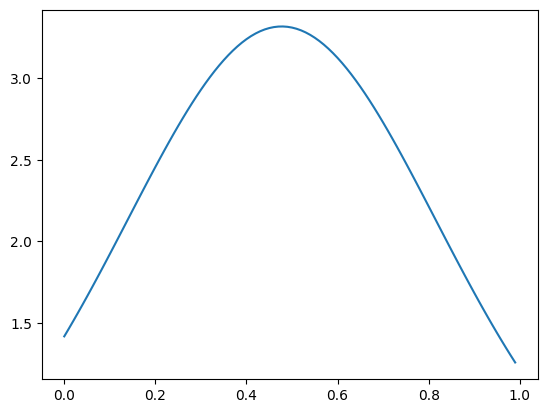
\includegraphics[width=\textwidth]{mu en fonction de z.png}
        \subcaption*{(a)}
        \label{fig:mu_z}
    \end{subfigure}
    \hfill
    \begin{subfigure}{0.45\textwidth}
        \centering
        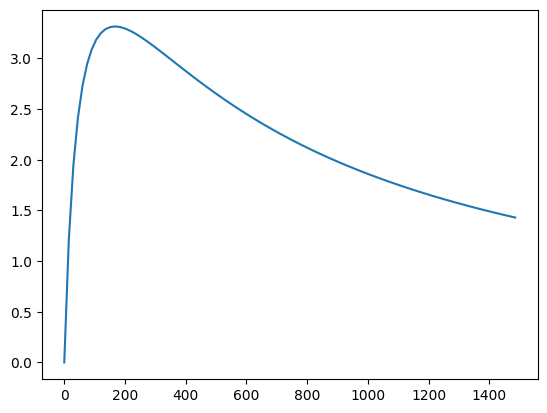
\includegraphics[width=\textwidth]{mu en fonction de I.png}
        \subcaption*{(b)}
        \label{fig:mu_I}
    \end{subfigure}

    \medskip

    \begin{subfigure}{0.45\textwidth}
        \centering
        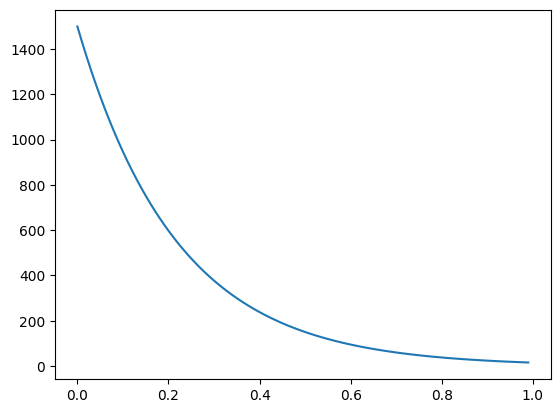
\includegraphics[width=\textwidth]{I en fonction de z.png}
        \subcaption*{(c)}
        \label{fig:I_z}
    \end{subfigure}

    \caption{
    (a) $\mu\,(d^{-1})$ as a function of $z$ ;
    (b) $\mu\,(d^{-1})$ as a function of $I$ ;
    (c) $I$ as a function of $z$
    }
    \label{fig:global}
\end{figure}


The simulations are performed for a single layer, and therefore without any mixing effects. 
The only varying parameter is the water velocity $u$. For a discretization of 500 points, we impose a uniform initial concentration and an initial total biomass of 50 Kg.
After an hour of growth, we get the following total biomass table for different current speed values.

\begin{table}[h!]
\centering
\begin{tabular}{|c|c|}
\hline
\textbf{Current speed (m.s$^{-1}$)} & \textbf{Total biomass (kg)} \\
\hline
0   & 52.8041 \\
0.1 & 52.6224 \\
0.2 & 52.6222 \\
0.3 & 52.6221 \\
0.5 & 52.6221 \\
1   & 52.6221 \\

\hline
\end{tabular}
\caption{Total biomass (T = 3600 s), as a function of current speed}
\label{tab:biomass_speed}
\end{table}

It seems, that the biomass grows less as the current increases. One must take into account that $\Delta_t$, the time step of the numerical scheme depends on the value of the speed $u$. 
This follows from the upwind scheme CFL condition. 


\section{Firt Optimization of the Mixing Matrix : The permutation case}

\subsection{General Principle of the Algorithm}

The objective of the algorithm is to optimize a mixing matrix applied to a discretized basin,
in order to maximize the total biomass produced by the system.

For a given initial configuration, a candidate mixing matrix is repeatedly applied to the system.
The temporal evolution of the basin is simulated with a constant time step, for a given period $T$.
The total biomass is then evaluated.

The algorithm explores different admissible mixing matrices (among every existing permutation matrices) and retains the one
that maximizes the final total biomass.

\subsection{Tested Initial Configurations}

In this study, the basin consists of three vertical layers.
The initial conditions are constructed by placing all the initial biomass (50 Kg) in a single layer,
while the other layers start with zero biomass. 
Three configurations are therefore considered, corresponding to the successive activation of each layer. The idea is to choose the mixing matrix which induces a maximal biomass after an hour of growth. 
We will set the current speed value $u$ to 0.3 $\mathrm{m\, s^{-1}}$. It is a rather small value, but as the CFL depends on it, a smaller speed value leads to a shorter computing time. 
300 seconds of growth therefore correspond to approximately 20 laps.

\subsection{Optimization Results}

For each initial configuration, the optimization algorithm converges to a matrix
that maximizes the final total biomass with T = 300 s.

\subsubsection{Comparative Analysis}

The optimization results show that the optimal mixing matrix depends strongly on the initial configuration of the basin.
When biomass is localized in an inherently favorable layer (with the highest growth rate),
keepig each layer unchanged is optimal (no mixing).
Conversely, in less favorable configurations,
vertical mixing allows biomass to be redistributed to more productive layers. We will see that the optimal matrices allocate biomass to the last layer (the deepest one).
Indeed, as $\mu = A\, I\, k_h\, \sigma_H$, the $\mu$ values of each layer are the following :

\begin{table}[H]
\centering
\begin{tabular}{|c|c|c|}
\hline
\textbf{Layer} & \textbf{$\mu$ (s$^{-1}$)} & \textbf{I} ($\mu$\text{mol} $m^{-2} s^{-1}$)\\
\hline
Layer 1 & $1.4198 \times 10^{-5}$ & 1500 \\
Layer 2 & $3.0538 \times 10^{-5}$ & 323.72 \\
Layer 3 & $2.8777 \times 10^{-5}$ & 69.86 \\
\hline
\end{tabular}
\caption{Growth rates $\mu$ for each initial layer configuration}
\label{tab:mu_layers}
\end{table}

Therefore the last layer has the biggest growth rate.

\subsubsection{Configuration 1: biomass initially in layer 1}

The maximal total biomass obtained is:
\[
B_{\text{tot}} = 50.301 \quad \mathrm{Kg}
\]

The optimal mixing matrix is:
\[
\mathbf{M}_1 =
\begin{pmatrix}
0 & 0 & 1 \\
1 & 0 & 0 \\
0 & 1 & 0
\end{pmatrix}
\]

This matrix induces a permutation of layers which induces the allocation of layer 1 in position 2, corresponding to the largest growth coefficient.
Here is a graphic representing the total algae mass in each layer as a function of time, with the latter permutation matrix.

\begin{figure}[H]
    \centering
    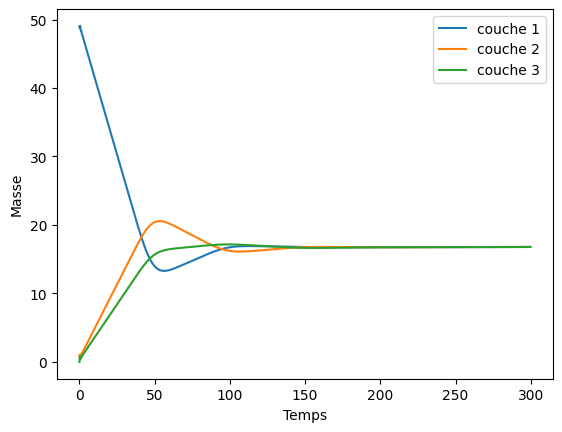
\includegraphics[width=0.5\textwidth]{masse_par_couche_N=3.png}
    \caption{biomass in each layer through time}
    \label{fig:t0}
\end{figure}

\subsubsection{Configuration 2: biomass initially in layer 2}

The maximal total biomass obtained is:
\[
B_{\text{tot}} = 50.461 \quad \mathrm{Kg}
\]

The optimal mixing matrix is:
\[
\mathbf{M}_2 =
\begin{pmatrix}
1 & 0 & 0 \\
0 & 1 & 0 \\
0 & 0 & 1
\end{pmatrix}
\]

Here, not mixing appears to be the optimal strategy.

\subsubsection{Configuration 3: biomass initially in layer 3}

The maximal total biomass obtained is:
\[
B_{\text{tot}} = 50.447 \quad \mathrm{Kg}
\]

The optimal mixing matrix is:
\[
\mathbf{M}_3 =
\begin{pmatrix}
1 & 0 & 0 \\
0 & 0 & 1 \\
0 & 1 & 0
\end{pmatrix}
\]

This configuration corresponds to the permutation of layers 2 and 3.

\subsection{other initial configurations, 5 layers}
\begin{table}[H]
\centering
\begin{tabular}{|c|c|c|}
\hline
\textbf{Layer} & \textbf{$\mu$ (s$^{-1}$)} & \textbf{I} ($\mu$\text{mol} $m^{-2} s^{-1}$)\\
\hline
Layer 1 & $1.4198 \times 10^{-5}$ & 1500 \\
Layer 2 & $2.4558 \times 10^{-5}$ & 597.8 \\
Layer 3 & $3.2373 \times 10^{-5}$ & 238.2 \\
Layer 4 & $3.1229 \times 10^{-5}$ & 94.94 \\
Layer 5 & $2.2153 \times 10^{-5}$ & 37.83 \\
\hline
\end{tabular}
\end{table}
\subsubsection{Configuration 1: biomass initially in layer 1}
After a period T= 300 $s$ of growth, the total biomass obtained is:
\[
B_{\text{tot}} = 50.390 \quad \mathrm{Kg}
\]

Optimal mixing matrix:
\[
\mathbf{M}_1 =
\begin{pmatrix}
0 & 0 & 0 & 1 & 0 \\
0 & 1 & 0 & 0 & 0 \\
1 & 0 & 0 & 0 & 0 \\
0 & 0 & 1 & 0 & 0 \\
0 & 0 & 0 & 0 & 1
\end{pmatrix}
\]
Here again, let us represent the successive biomass values associated to the tested permutation matrices :

\begin{figure}[H]
\centering
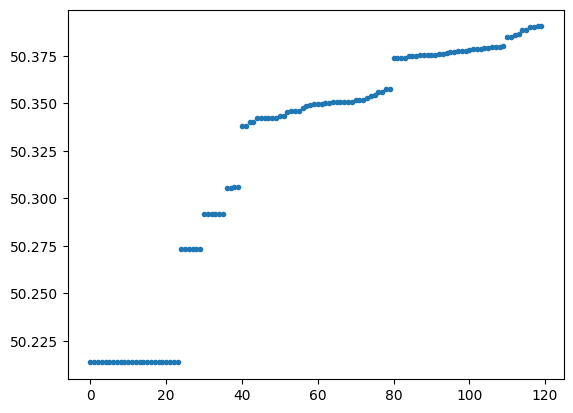
\includegraphics[width=0.6\textwidth]{biomasses recherche matrice N=5.png}
\end{figure}
\subsubsection{Configuration 2: biomass initially in layer 2}

Total biomass obtained:
\[
B_{\text{tot}} = 50.443 \quad \mathrm{Kg}
\]

Optimal mixing matrix:
\[
\mathbf{M}_2 =
\begin{pmatrix}
1 & 0 & 0 & 0 & 0 \\
0 & 0 & 0 & 1 & 0 \\
0 & 1 & 0 & 0 & 0 \\
0 & 0 & 1 & 0 & 0 \\
0 & 0 & 0 & 0 & 1
\end{pmatrix}
\]

\subsubsection{Configuration 3: biomass initially in layer 3}

Total biomass obtained:
\[
B_{\text{tot}} = 50.488 \quad \mathrm{Kg}
\]

Optimal mixing matrix:
\[
\mathbf{M}_3 =
\begin{pmatrix}
1 & 0 & 0 & 0 & 0 \\
0 & 1 & 0 & 0 & 0 \\
0 & 0 & 1 & 0 & 0 \\
0 & 0 & 0 & 1 & 0 \\
0 & 0 & 0 & 0 & 1
\end{pmatrix}
\]

\subsubsection{Configuration 4: biomass initially in layer 4}

Total biomass obtained:
\[
B_{\text{tot}} = 50.480 \quad \mathrm{Kg}
\]

Optimal mixing matrix:
\[
\mathbf{M}_4 =
\begin{pmatrix}
0 & 1 & 0 & 0 & 0 \\
1 & 0 & 0 & 0 & 0 \\
0 & 0 & 0 & 1 & 0 \\
0 & 0 & 1 & 0 & 0 \\
0 & 0 & 0 & 0 & 1
\end{pmatrix}
\]

\subsubsection{Configuration 5: biomass initially in layer 5}

Total biomass obtained:
\[
B_{\text{tot}} = 50.431 \quad \mathrm{Kg}
\]

Optimal mixing matrix:
\[
\mathbf{M}_5 =
\begin{pmatrix}
1 & 0 & 0 & 0 & 0 \\
0 & 1 & 0 & 0 & 0 \\
0 & 0 & 0 & 0 & 1 \\
0 & 0 & 1 & 0 & 0 \\
0 & 0 & 0 & 1 & 0
\end{pmatrix}
\]
\section{Mixing Optimization : Optimal Stochastic Mixing-Matrix}

Now that we have found a way to determine the best permutation matrix for the water pond, let us now focus on a more general case : the column stochastic matrices. 
The initial problem is indeed defined with $P$ a $N \times N$ column-stocastic matrix. To optimize on this infinite space, we will have to use a differentiable program.
We have chosen the torch python library to do so. In the update fonction, we have to convert every numpy list and array into a torch variable. This will allow us to compute torch differentiation with these variables. 
Furthermore, to process the matrix constraints (non negative coefficients and every column must sum 1), we will use the softmax function, in order to differentiate with respect an unconstrained matrix $Q$.

The objective function remains the same.

\subsection{Optimal stochastic matrix}


Let us now use the original objective function, i.e the final biomass after a given growth period $T$. 
As before, the growth time remains $T = 300 s$ and the initial conditions are that the total biomass is in layer 1. The algorithm complexity is a linear function of the number of layers.
Therefore, it allows us to divide the water pond in 10 layers. 

\subsubsection{optimizer parameters}

The Adam optimizer (Adaptive Moment Estimation) combines momentum-based gradient descent with per-parameter adaptive learning rates. 
At each iteration $t$, it maintains an exponential moving average of the gradient $m_t$ (first moment) and of the squared gradient $v_t$ (second moment), defined as
\[
m_t = \beta_1 m_{t-1} + (1-\beta_1) g_t, \qquad
v_t = \beta_2 v_{t-1} + (1-\beta_2) g_t^2,
\]
where $g_t$ denotes the gradient of the loss with respect to the parameters. These moment estimates are corrected for initialization bias as
\[
\hat m_t = \frac{m_t}{1-\beta_1^t}, \qquad
\hat v_t = \frac{v_t}{1-\beta_2^t}.
\]
The parameter update is then given by
\[
\theta_{t+1} = \theta_t - \alpha \frac{\hat m_t}{\sqrt{\hat v_t} + \varepsilon},
\]
where $\alpha$ is the global learning rate, while $\beta_1$ and $\beta_2$ control the exponential decay rates of the first and second moments, respectively, governing the trade-off between stability and responsiveness of the optimization process.

In order to choose an appropriate learning rate for the Adam optimization algorithm, we performed a learning rate finder experiment. The principle consists in lauching the optimization with different $\alpha$ values, and check which one converges the quickest. 

\begin{figure}[H]
\centering
    \begin{subfigure}{0.3\textwidth}
        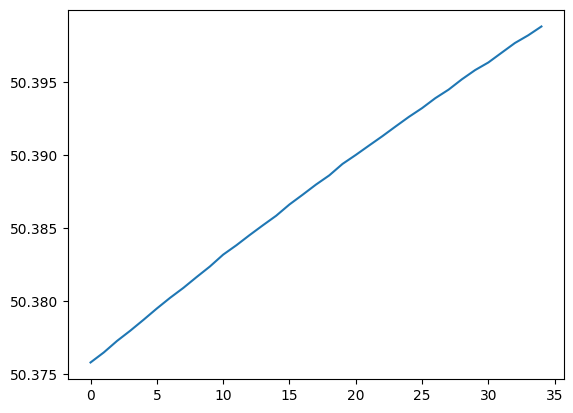
\includegraphics[width=\textwidth]{convergence stocha, N=10, lr=0.01.png}
        \subcaption*{(a)}
        \label{fig:lr_0.01}
    \end{subfigure}
    \hfill
    \begin{subfigure}{0.3\textwidth}
        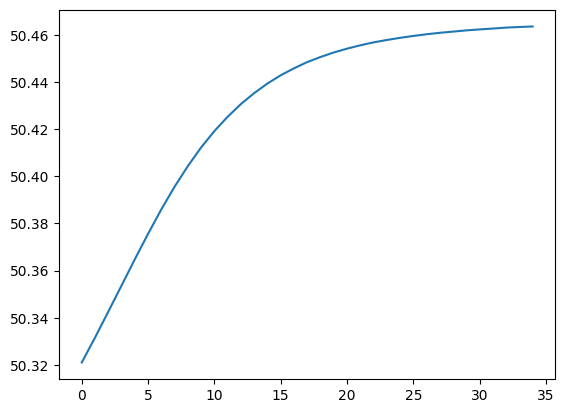
\includegraphics[width=\textwidth]{convergence stocha, N=10, lr=0.1.png}
        \subcaption*{(b)}
        \label{fig:lr_0.1}
    \end{subfigure}
    \hfill
    \begin{subfigure}{0.3\textwidth}
        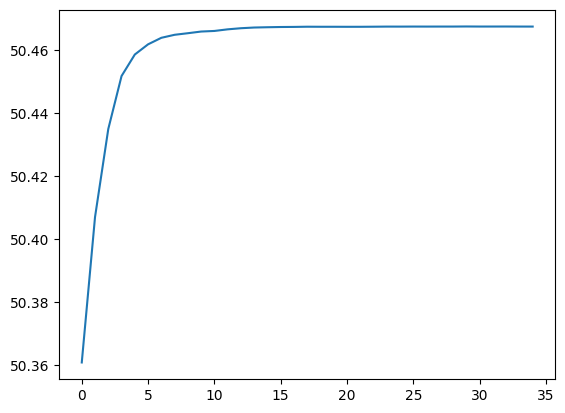
\includegraphics[width=\textwidth]{convergence stocha, N=10, lr=0.9.png}
        \subcaption*{(c)}
        \label{fig:lr_0.9}
    \end{subfigure}
    \caption{
    (a) $\alpha = 0.01$;
    (b) $\alpha = 0.1$ ;
    (c) $\alpha = 0.9$
    }
    \label{fig:global}
\end{figure}

It is clear that the best learning rate is $\alpha = 0.9$. It reaches a plateau after about 12 iterations. Based on this observation, we can arbitrarely bond the number of iterations by 12.

For 10 layers, the approximate optimal matrix is the following.

\[
\begin{pmatrix}
0.000 & 0.003 & 0.010 & 0.000 & 0.000 & 0.000 & 0.001 & 0.001 & 0.001 & 0.004 \\
0.000 & 0.011 & 0.001 & 0.020 & 0.000 & 0.000 & 0.000 & 0.007 & 0.004 & 0.006 \\
0.000 & 0.009 & 0.008 & 0.003 & 0.000 & 0.000 & 0.000 & 0.005 & 0.004 & 0.004 \\
0.001 & 0.394 & 0.373 & 0.080 & 0.000 & 0.000 & 0.002 & 0.112 & 0.151 & 0.082 \\
0.003 & 0.285 & 0.251 & 0.072 & 0.012 & 0.000 & 0.504 & 0.073 & 0.193 & 0.051 \\
0.992 & 0.095 & 0.076 & 0.443 & 0.985 & 0.999 & 0.345 & 0.511 & 0.331 & 0.599 \\
0.003 & 0.087 & 0.140 & 0.371 & 0.001 & 0.000 & 0.142 & 0.283 & 0.268 & 0.203 \\
0.000 & 0.103 & 0.131 & 0.005 & 0.001 & 0.000 & 0.005 & 0.001 & 0.041 & 0.045 \\
0.000 & 0.007 & 0.005 & 0.006 & 0.000 & 0.000 & 0.000 & 0.001 & 0.001 & 0.002 \\
0.000 & 0.007 & 0.006 & 0.000 & 0.000 & 0.000 & 0.000 & 0.005 & 0.005 & 0.002
\end{pmatrix}
\]

As seen before, the line 6 has the largest coefficients because layer 6 has the highest growth coefficient. The optimal matrix allocates most of the biomass in this layer.
But stochastic matrices aren't physically relevant. Indeed, in terms of water volume, a real-life paddle wheel should allocate to each layer exactly the volume of one layer. 
Such a wheel could only be represented by a bistochastic matrix.

\section{Optimal bistochastic matrix}

Using the same solver than before, we only add a penalty to the objective function to impose that the sum on each line of the mixing matrix should equal 1.
After lauching the program for a $10$ layers pond, we end up with the following matrix.

\[
\begin{bmatrix}
0.1727 & 0.0401 & 0.1280 & 0.1118 & 0.0686 & 0.0839 & 0.0447 & 0.2331 & 0.0285 & 0.0885 \\
0.0422 & 0.2675 & 0.0660 & 0.1765 & 0.0297 & 0.0281 & 0.1194 & 0.1010 & 0.0907 & 0.0790 \\
0.2268 & 0.0297 & 0.1286 & 0.0654 & 0.0687 & 0.0290 & 0.2182 & 0.0791 & 0.1469 & 0.0075 \\
0.1335 & 0.1178 & 0.0531 & 0.0894 & 0.1766 & 0.0053 & 0.0866 & 0.0164 & 0.0864 & 0.2348 \\
0.2559 & 0.0255 & 0.3115 & 0.0160 & 0.0122 & 0.0688 & 0.0067 & 0.1059 & 0.1850 & 0.0123 \\
0.0238 & 0.3348 & 0.0341 & 0.0567 & 0.2197 & 0.0715 & 0.0415 & 0.0387 & 0.1417 & 0.0375 \\
0.0467 & 0.0217 & 0.0830 & 0.3417 & 0.0783 & 0.0183 & 0.2618 & 0.0856 & 0.0249 & 0.0380 \\
0.0410 & 0.0510 & 0.0688 & 0.0451 & 0.2185 & 0.1392 & 0.0301 & 0.2752 & 0.1097 & 0.0213 \\
0.0356 & 0.0181 & 0.0586 & 0.0700 & 0.1100 & 0.5202 & 0.0761 & 0.0173 & 0.0743 & 0.0198 \\
0.0218 & 0.0936 & 0.0683 & 0.0274 & 0.0177 & 0.0357 & 0.1148 & 0.0476 & 0.1119 & 0.4613
\end{bmatrix}
\]

This mixing matrix corresponds to a final biomass (after $T = 300s$ of growth) of $B_{\text{tot}} = 50.369 \quad \mathrm{Kg}$.

Let us try to launch the algorithm with an initial permutation matrix. We notice that it converges with a similar pattern for each matrix. 
For example, starting from the identity, the algorithm returns the following matrix.

\[
\begin{pmatrix}
0.2263 & 0.0860 & 0.0861 & 0.0859 & 0.0859 & 0.0860 & 0.0859 & 0.0859 & 0.0861 & 0.0859 \\
0.0841 & 0.2321 & 0.0856 & 0.0855 & 0.0855 & 0.0855 & 0.0855 & 0.0855 & 0.0855 & 0.0854 \\
0.0867 & 0.0863 & 0.2309 & 0.0850 & 0.0850 & 0.0850 & 0.0850 & 0.0850 & 0.0847 & 0.0863 \\
0.0865 & 0.0850 & 0.0853 & 0.2317 & 0.0853 & 0.0853 & 0.0853 & 0.0852 & 0.0852 & 0.0850 \\
0.0873 & 0.0850 & 0.0852 & 0.0852 & 0.2316 & 0.0852 & 0.0852 & 0.0852 & 0.0851 & 0.0850 \\
0.0875 & 0.0849 & 0.0852 & 0.0852 & 0.0852 & 0.2315 & 0.0852 & 0.0851 & 0.0851 & 0.0849 \\
0.0870 & 0.0850 & 0.0852 & 0.0852 & 0.0852 & 0.0852 & 0.2316 & 0.0852 & 0.0851 & 0.0850 \\
0.0860 & 0.0851 & 0.0853 & 0.0853 & 0.0853 & 0.0853 & 0.0853 & 0.2319 & 0.0852 & 0.0850 \\
0.0849 & 0.0853 & 0.0855 & 0.0854 & 0.0854 & 0.0854 & 0.0854 & 0.0854 & 0.2322 & 0.0853 \\
0.0835 & 0.0854 & 0.0856 & 0.0855 & 0.0856 & 0.0856 & 0.0856 & 0.0855 & 0.0856 & 0.2322
\end{pmatrix}
\]

wich is an affine translation of the identity. But the final biomass is lower than the one associated with the first matrix : starting the gradient descent from the identity brings us to a local maximum of $B_{\text{tot}} = 50.357 \quad \mathrm{Kg}$.
There seems to be a local maximum of the objective function "near" each permutation matrix. As observed in simulations, launching the gradient descent with a permutation matrix $P$ will converge to a bistochastic matrix close to :
\[ 0.086*E + 0.14*P\] where $E = (1)_{1\leq i, j \leq I}$.



\section{research perspectives and next steps in the work plan}
As an immediate next step, we can compute this algorithm starting from different types of bistochastic matrices, to get a better idea of the surface generated by the function on the set of bistochastic matrices. Furthermore, we could try to find a way to associate a matrix to a real-life paddle wheel to try and compare the optimization results to reality.

\section{annexes}
\subsection{initial test}
To check if the new solver is functional. In order to do so, let us consider a three layers basin, and an objective function which mixes these layers with respect to the matrix $P = \text{softmax}(Q)$ and returns the total biomass, after a pre-determined growing period. 
The growth coefficients will be arbitrarely set to 1 for layer 1, 2 for layer 2 and 3 for layer 3. Therefore, with an initial basin in which the total biomass is concentrated in layer 1, an optimal matrix should reallocate it in layer 3. 
Let us consider the results.

The optimal mixing matrix is:
\[
\mathbf{P} =
\begin{pmatrix}
0.003 & 0.50 & 0.26 \\
0.007& 0.30 & 0.10\\
0.99 & 0.20 & 0.64
\end{pmatrix}
\]

The first layer is indeed moved to layer 3 by 99 percent. 

\subsection{3 layers comparison test}
With an initial pond of 3 layers, in which the biomass is only in the first layer, the solver returns the following matrix :
\[
\begin{pmatrix}
4.126\times 10^{-5} & 3.704\times 10^{-4} & 2.707\times 10^{-4} \\
9.961\times 10^{-1} & 9.976\times 10^{-1} & 9.848\times 10^{-1} \\
3.901\times 10^{-3} & 2.034\times 10^{-3} & 1.495\times 10^{-2}
\end{pmatrix}
\]


this matrix corresponds to a situation in which the final biomass is $50.301 \text{Kg}$. This is approximately the same result than the permutation matrix case. 
The optimal permutation matrix was indeed :
\[
\mathbf{M}_1 =
\begin{pmatrix}
0 & 0 & 1 \\
1 & 0 & 0 \\
0 & 1 & 0
\end{pmatrix}
\]
We can now begin the ADAM algorithm starting from this matrix and see if we obtain a better result. The final biomass result stays the same, while the optimisation returns a new matrix :
\[
\begin{pmatrix}
7.768 \times 10^{-4} & 3.514 \times 10^{-4} & 3.007 \times 10^{-3} \\
9.933 \times 10^{-1} & 9.974 \times 10^{-1} & 9.429 \times 10^{-1} \\
5.955 \times 10^{-3} & 2.301 \times 10^{-3} & 5.411 \times 10^{-2}
\end{pmatrix}
\]
\subsection{Newton method}
Let us try to use another optimizer, based on the Newton method with conjugate gradient.
This method is a second-order optimization technique used to find a local minimizer of a twice-differentiable function $f : \mathbb{R}^n \to \mathbb{R}$. 
At iteration $k$, the Newton direction $p_k$ is defined as the solution of the linear system
\[
\nabla^2 f(x_k) p_k = -\nabla f(x_k),
\]
where $\nabla f(x_k)$ is the gradient and $\nabla^2 f(x_k)$ is the Hessian matrix.

For large-scale problems as ours, explicitly forming and inverting the Hessian matrix is computationally expensive. 
Instead, the Newton system can be solved approximately using the Conjugate Gradient (CG) method. 
The CG algorithm is particularly efficient when the Hessian is symmetric and positive definite, as it only requires matrix-vector products.

In the Newton-CG method, at each iteration we apply the Conjugate Gradient algorithm to compute an approximate solution $p_k$ of the Newton system. 
The iterate is then updated as
\[
x_{k+1} = x_k + \alpha_k p_k,
\]
where $\alpha_k$ is determined by a line search procedure.
\subsection{Computational complexity.}

We analyze the computational complexity of the optimization procedure by first estimating the cost of a single evaluation of the objective function. The time step of the numerical scheme is given by
\[
\Delta t = \mathrm{CFL}\,\frac{\Delta x^2}{2\mu + a\,\Delta x},
\quad \text{with} \quad \Delta x = \frac{L}{n},
\]
where $n$ denotes the number of spatial discretization points, $\mu$ the diffusion coefficient, and $a$ a characteristic advection velocity. Substituting $\Delta x$ yields
\[
\Delta t
= \mathrm{CFL}\,\frac{L^2}{n^2(2\mu + aL/n)}
= \frac{\mathrm{CFL}\,L^2}{2\mu n^2 + aLn}.
\]

In our setting, typical parameter values are $\mu \approx 10^{-5}$, $n \approx 50$, $0.01 < a < 0.1$, and $L \approx 5$. Under these assumptions, the term $aLn$ dominates $2\mu n^2$, leading to the approximation
\[
\Delta t \sim \frac{\mathrm{CFL}\,L}{a\,n}.
\]

The objective function corresponds to the final state of a time-marching simulation over a time horizon $T$. The number of time steps is therefore of order $T / \Delta t$, and each time step involves $O(Nn)$ operations, where $N$ denotes the number of layers. Consequently, the computational complexity of a single forward evaluation of the objective function is
\[
\mathcal{O}\!\left( Nn \frac{T}{\Delta t} \right)
= \mathcal{O}\!\left( \frac{a\,N\,n^2\,T}{\mathrm{CFL}\,L} \right).
\]

Since the objective function is implemented in a differentiable manner using automatic differentiation, the backward pass requires propagating gradients through the entire time-marching scheme. The computational cost of the backward pass is of the same order as the forward pass, up to a constant factor, yielding
\[
\mathcal{O}\!\left( \frac{a\,N\,n^2\,T}{L} \right).
\]

Finally, the full optimization procedure consists of $K$ iterations of the Adam algorithm. Each iteration requires one forward evaluation of the objective function and one backward pass, while the update of the parameter matrix $P \in \mathbb{R}^{N \times N}$ is negligible in comparison. The overall computational complexity of the \texttt{solve} algorithm is therefore
\[
\mathcal{O}\!\left( K\,\frac{a\,N\,n^2\,T}{L} \right).
\]

\begin{thebibliography}{9}

\bibitem{1}
Liu-Di Lu,
\textit{Lagrangian Approaches for Modelling
and Optimization of
Hydrodynamic-Photosynthesis
Coupling},
Sorbonne Université, LJLL, 2021
\bibitem{2}
Oxford reference
\textit{Beer-Lambert Law}
\end{thebibliography}
\end{document}